% Chapter 3

\chapter{Image Reconstruction} % Main chapter title

\label{Chapter3} % For referencing the chapter elsewhere, use \ref{Chapter3} 

\lhead{Chapter 3. \emph{Image Reconstruction}} % This is for the header on each page - perhaps a shortened title

%----------------------------------------------------------------------------------------

%----------------------------------------------------------------------------------------
\section{The Van Cittert-Zernike theorem}\
\label{sec:about3}
As seen in chapter~\ref{Chapter1} and chapter~\ref{Chapter2}, the interferometer measures the complex visibility, $V'(u,v)$, of a source, which is the Fourier transform of its intensity distribution multiplied by the primary beam response as observed in the equations,~\ref{eq:visEq} and~\ref{eq:VisOut0}. The true visibility, $V(u,v)$ can be expressed as follows~\citep[Slide 8]{jdf.webinar.2}:
\begin{equation}
\label{eq:visiPhase}
	V(u,v) = |V|e^{-j\phi} = \iint{I(l,m)e^{-j2\pi{(ul +vm)}}dldm} 
%{{\sqrt{1 - l^2 - m^2}}}
\end{equation}
The Fourier transform relationship between the true visibility, $V(u,v)$, and the sky intensity distribution, $I(l,m)$, is the Van Cittert-Zernike theorem on which synthesis imaging is based.
This means that we can recover $I(l,m)$ from $V(u,v)$: 
\begin{align}
V(u,v) &=& &\iint{I(l,m){e^{-2j\pi{(ul +vm)}}} dldm}\\
I(l,m) &=& &\iint{V(u,v){e^{2j\pi{(ul +vm)}}} dudv}
\end{align}
\begin{figure}[htbp]
\center
    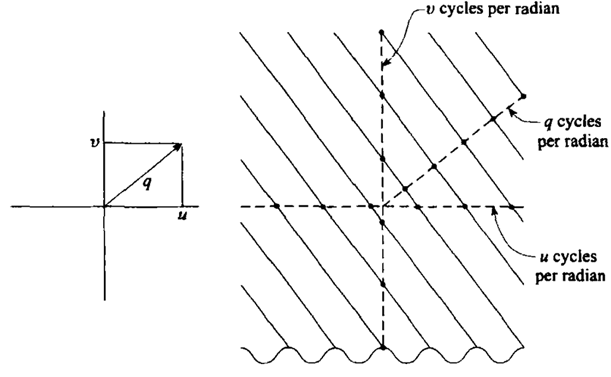
\includegraphics[scale= 0.3]{Figures/phaseQ}
 	\caption[Fringe Visibility]{Fringe Visibility~\citep[Pg. 64,~Fig. 2.7]{thompson2008interferometry}}
	\label{fig:VisiPhaseQ}
\end{figure}
In eq.~\ref{eq:visiPhase}, the visibility is expressed as, $|V|e^{-j\phi}$. The phase, $\phi$, contains information about the location of structure with spatial frequency $(u,v)$ relative to the phase centre $(l=0,m=0)$, and the amplitude, $|V|$, gives information about how much of the spatial frequency component is present~\citep[Slide 8]{jdf.webinar.2}~\citep[Slide 9]{wilner.siw2014}.\\ 
\begin{figure}[htbp]
\center
    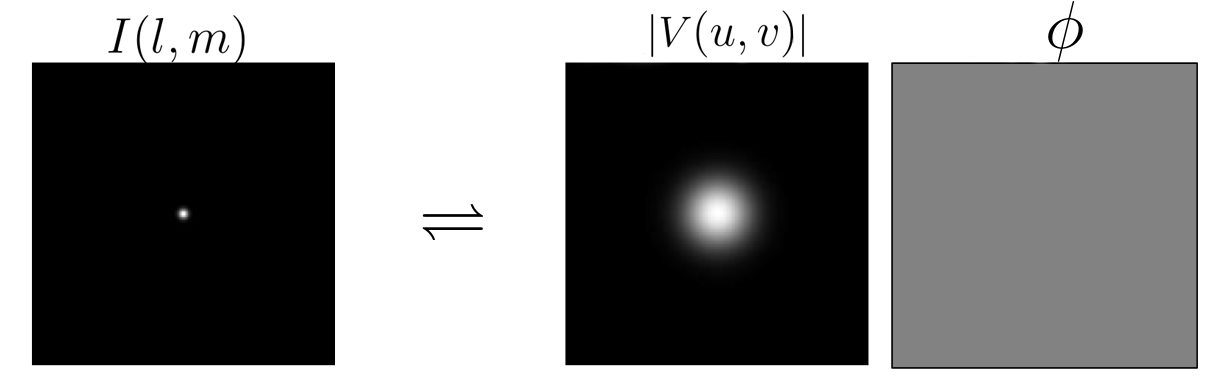
\includegraphics[scale= 0.3]{Figures/phase0}
 	\caption[Amplitude and fringe of the visibility function]{Amplitude and fringe of the visibility function, source at phase centre~\citep[Slide 9]{wilner.siw2014}}
	\label{fig:VisiPhase0}
\end{figure}
\begin{figure}[htbp]
\center
    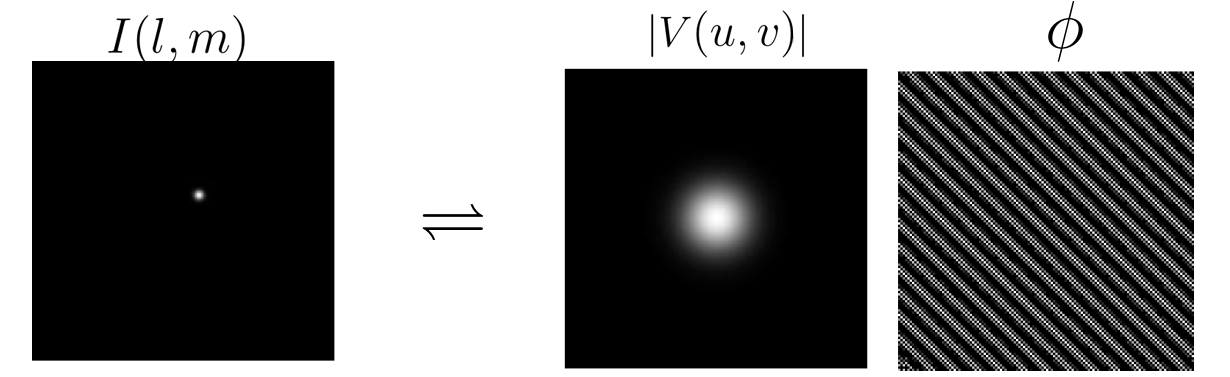
\includegraphics[scale= 0.3]{Figures/phase1}
 	\caption[Amplitude and fringe of the visibility function, where the source is offset the phase centre]{Amplitude and fringe of the Visibility function source offset from the phase centre in the upper-right direction~\citep[Slide 9]{wilner.siw2014}}
	\label{fig:VisiPhase1}
\end{figure}
\section{Sampling of the visibility}
We already know about the visibility from the previous sections, and chapter~\ref{Chapter2} which showed how it can be obtained for a pair of antennas. Now consider the following, let us denote the baseline vector components for a particular interferometer antenna-pair, that we index $(i,k)$, as $(u_{ik},v_{ik})$. For a single measurement of cross-correlation of the voltages, $V_i(t)$, and, $V_k(t)$, from the interferometer, e.g. $V_i{\star}V_k$, we get a value which relates to the visibility value, $V(u_{ik},v_{ik})$, however though a fairly important property of the visibility function, $V(u,v)$, is that it is hermitian~\citep[Pg. 138,~Sec.~5.4]{thompson2008interferometry}, so for the example we mentioned, we can write the following:
\begin{equation}
\label{eq:hermiVis}
V(u_{ik},v_{ik}) = V^{*}(-u_{ik},-v_{ik})
\end{equation}
Thus for one measurement with a particular pair of antennas we can obtain data about $V(u,v)$ at two positions on the $u-v$ plane as one can see from equation~\ref{eq:hermiVis}, its like the interferometer acts as a filter~\citep[Pg. 133,~Sec.~5.3]{thompson2008interferometry} that responds to spatial frequencies $(u_{ik},v_{ik})$ and $(-u_{ik},-v_{ik})$. Ultimately what we want is to obtain an appropriate coverage of the  $u$-$v$ plane, so we need to have different baselines to be able to accomplish this, usually this is done by having an array of antennas, or by having adjustable baselines or/and also using earth rotation synthesis which we'll discuss later, and the choice of configuration of the antennas of a synthesis array is based on optimising, in some manner, the sampling of the visibility function in $(u,v)$ space~\citep[Pg. 126,~Sec.~5.2]{thompson2008interferometry}.\\

\subsection{Sampling Theorem}
\label{sec:sampTheo}
\begin{figure}[htbp]
\center
    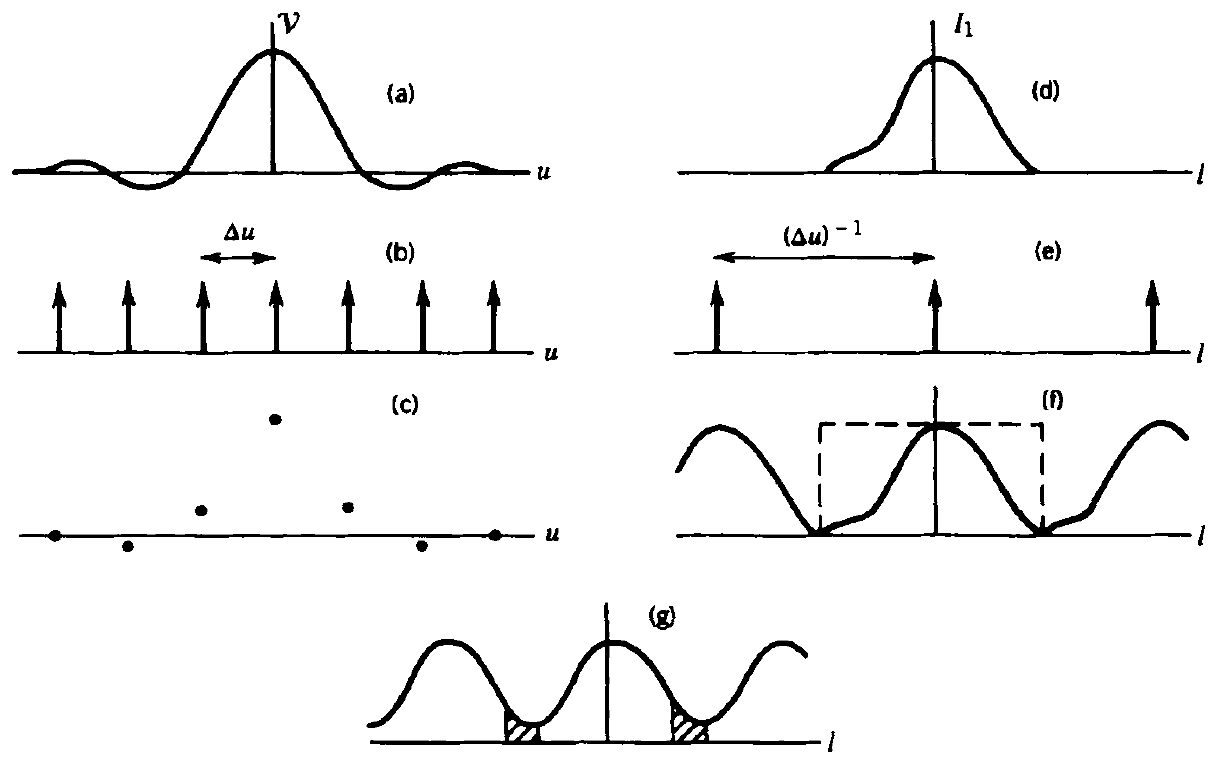
\includegraphics[scale= 0.3]{Figures/sampling}
 	\caption[Sampling a 1-D visibility  ]{Sampling a 1-D visibility~\citep[Pg.~126,~Fig.~5.2]{thompson2008interferometry}}
	\label{fig:Sampling1D}
\end{figure}
{\citep[From][~Sec.~5.2]{thompson2008interferometry}}~Now to appreciate the effect of sampling and its requirement let's focus on the following example, in which one wants to measure the one-dimensional intensity distribution of a source, $I(l,0)$, portrayed in Fig.~\ref{fig:Sampling1D}{\color{blue}(d)}. It is necessary to measure the complex visibility, $V$, in the corresponding direction on the ground at a series of values of the projected antenna spacing. For example, to measure an east-west profile, a possible method is to make observations near meridian transit of the source using an east-west baseline, and to vary the length of the baseline from day to day~\citep[Pg. 126]{thompson2008interferometry}, or have an array of antennas with baselines which have multiples of a unit spacing, $\Delta{u}$. So we can represent the sampling as the multiplication of the visibility function with the impulse train function (familiar to the students), $\Sha_{\Delta{u}}(u)$, defined as follows,
\begin{equation}
\Sha_{\Delta{u}}(u) = \sum^{\infty}_{i = -\infty}\delta(u - i\Delta{u})\textrm{~\citet*{wiki:diracComb}}
\end{equation}

Thus the sampled, $V$, corresponds to the following,
\begin{equation}
S(u)\cdot{V(u,0)} = \Sha_{\Delta{u}}(u)\cdot{V(u,0)} = \sum^{\infty}_{i = -\infty}\delta(u - i\Delta{u}){\cdot}{V(u,0)}
\end{equation}
where, $S$, represents the general sampling function,
now the Fourier transform of the impulse function is the following{~\citep[Pg. 127,~Eq.~5.6]{thompson2008interferometry}},
\begin{equation}
\Sha_{\Delta{u}}(u) \rightleftharpoons \Sha_{\Delta{u}^{-1}}(l) = \sum^{\infty}_{i = -\infty}\delta(l - \frac{i}{\Delta{u}})
\end{equation}

as per the usual property of scaling for Fourier transforms. And from the convolution theorem. 

\begin{equation}
\Sha_{\Delta{u}}(u)\cdot{V(u,0)} \rightleftharpoons \Sha_{\Delta{u}^{-1}}(l)\ast{I(l,0)}
\end{equation}
{\citep[From][Pg. 127,~Sec.~5.2]{thompson2008interferometry}}~The result is the replication of, $I(l,0)$, at intervals $\Delta{u}^{-1}$ as observed in Fig.~\ref{fig:Sampling1D}{\color{blue}(f)}.
If, $I(l,0)$, represents a source of finite dimensions, the replications of
$I(l,0)$ will not overlap as long as $I(l,0)$ is nonzero only within a range of $l$ that
is no greater than $\Delta{u}^{-1}$. An example of overlapping replications is shown in
Fig.~\ref{fig:Sampling1D}{\color{blue}(g)}. The loss of information resulting from such overlapping is commonly referred to as aliasing, because the components of the function within the overlapping region lose their identity with respect to which end of the replicated function they properly belong. Avoidance of aliasing requires that the sampling interval $\Delta{u}$ be no greater than the reciprocal of the interval in $l$ within which $I(l,0)$ is nonzero. To be precise, we should consider the width of the source as broadened by the finite resolution of the observations, rather than the true width of the source,
but this is usually only a minor effect. The requirement for the restoration of a function from a set of samples, for example, deriving the function in Fig.~\ref{fig:Sampling1D}{\color{blue}(a)} from the samples in Fig.~\ref{fig:Sampling1D}{\color{blue}(c)} is easily understood by considering the Fourier transforms in Fig.~\ref{fig:Sampling1D}{\color{blue}(d)} and {\color{blue}(f)}. Interpolation in the $u$ domain corresponds to removing the replications in the $l$ domain, which can be achieved by multiplication of the function in Fig.~\ref{fig:Sampling1D}{\color{blue}(f)} by the rectangular function, $\Pi_{\Delta{u}^{-1}}(l)$ indicated by the broken line. In terms of the heavyside or unit step function, $\textrm{H}(l)$, (more familiar to the student) the rectangular function can be expressed as the following{~\citep{pjbevel.Box}},
\begin{equation}\Pi_{\Delta{u}^{-1}}(l) = \textrm{H}(l+\frac{\Delta{u}^{-1}}{2})- \textrm{H}(l - \frac{\Delta{u}^{-1}}{2})
\end{equation}
In the $u$ domain this multiplication corresponds to the convolution of the sampled values with the Fourier transform of the rectangular function, 

\begin{equation}
\Pi_{\Delta{u}^{-1}}(l) \rightleftharpoons {\Delta{u}^{-1}}\cdot\textrm{sinc}(u/{\Delta{u})}
\end{equation}

where, $\textrm{sinc}(x)$, is the normalised sinc function,
\begin{equation}
\textrm{sinc}(x) = \frac{\sin(\pi{x})}{\pi{x}}
\end{equation}

\begin{equation}
\Pi_{\Delta{u}^{-1}}(l) \rightleftharpoons \frac{\sin(\pi{u/{\Delta{u}})}}{\pi{u}}
\end{equation}
If aliasing is avoided, convolution with $\frac{\sin(\pi{u/{\Delta{u}})}}{\pi{u}}$ provides exact interpolation of the original function from the samples. Thus we can state, as a sampling theorem for the visibility, that if the intensity distribution is nonzero only within an interval of width, $l_w$, $I(l,0)$ is fully specified by sampling the visibility function at points spaced $\Delta{u} = l_w^{-1}$ in $u$. In two dimensions, it is simply necessary to apply the theorem separately to the source in the $l$ and $m$ directions{~\citep[Pg. 127]{thompson2008interferometry}}~.\\
\begin{figure}[htbp]
\center
    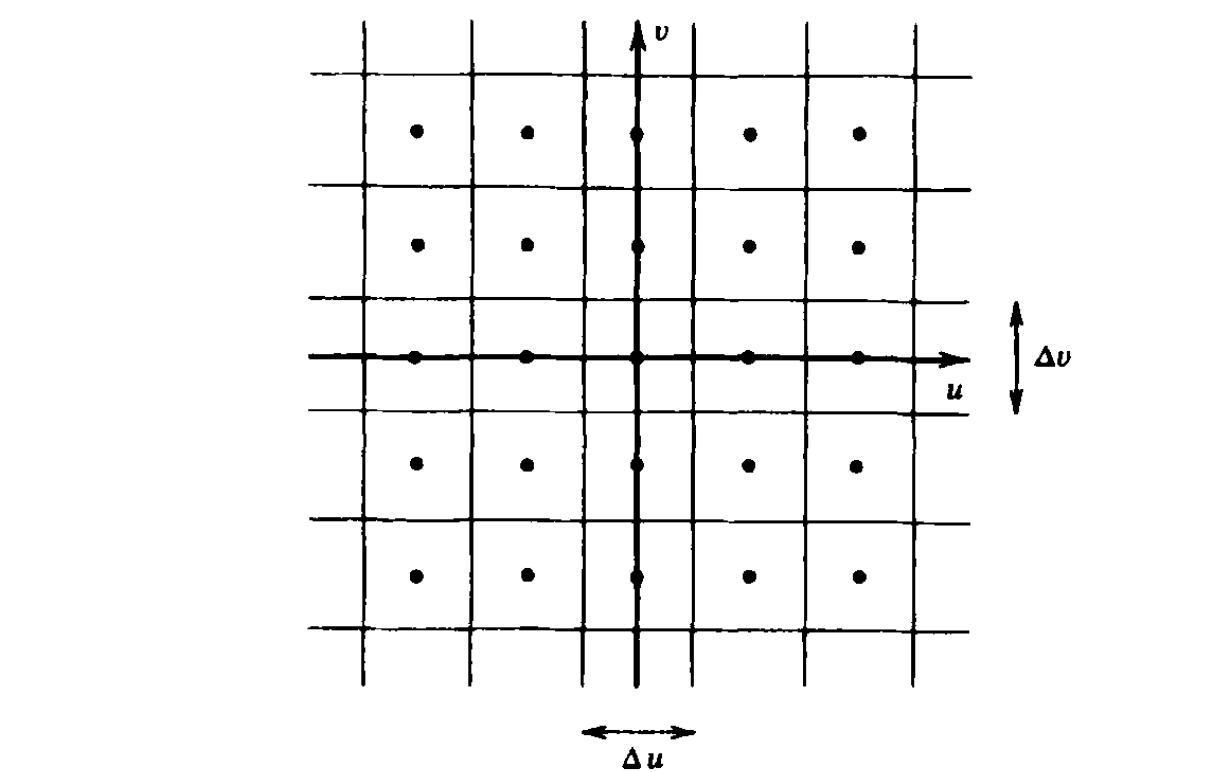
\includegraphics[scale= 0.3]{Figures/sampling2d}
 	\caption[Sampling a 2-D visibility  ]{Sampling a 2-D visibility~\citep[Pg.~129,~Fig.~5.3]{thompson2008interferometry}}
	\label{fig:Sampling2D}
\end{figure}
{~\citep[From][Pg. 128,~Sec.~5.2]{thompson2008interferometry}}~The discrete form of the Fourier transform is very widely used in synthesis mapping because of the computational advantages of the fast Fourier transform (FFT) algorithm. With the discrete transform the functions $V(u, v )$ and $I(l , m)$ are expressed as rectangular matrices of sampled values at uniform increments in the two variables involved. The rectangular grid points on which the intensity is obtained provide a convenient form for further data processing. The two-dimensional form of the discrete transform for the Fourier pair $V(u,v)$ and $I(l,m)$ is defined by,
\begin{equation}
\label{eq:Vdft}
V(p\Delta{u},q\Delta{v}) = \frac{1}{MN}\sum^{M-1}_{i = 0}\sum^{N-1}_{k=0}I(i\Delta{l},k\Delta{m}){e^{-j2\pi{ip}/M}}{e^{-j2\pi{kq}/N}}
\end{equation}
and the inverse is
\begin{equation}
\label{eq:Iidft}
I(i\Delta{l},k\Delta{m})= \frac{1}{MN}\sum^{M-1}_{p = 0}\sum^{N-1}_{q=0}V(p\Delta{u},q\Delta{v}) {e^{j2\pi{ip}/M}}{e^{j2\pi{kq}/N}}
\end{equation}
The functions are periodic with periods of $M$ samples in the $i$ and $p$ dimensions and $N$ samples in the $k$ and $q$ dimensions. Evaluation of Eqs.~\ref{eq:Vdft} or~\ref{eq:Iidft} by direct computation requires approximately $(MN)^2$ complex multiplications. In contrast, if $M$ and $N$ are powers of 2 the FFT algorithm requires only $\frac{1}{2}MN\log_2(MN)$ complex multiplications. The dimensions of the $(u ,v)$ plane that contain these data are $M\Delta{u}$ by $N\Delta{v}$. In the $(l,m)$ plane the points are spaced $\Delta{l}$ in $l$ and $\Delta{m}$ in $m$, and the map dimensions are $M\Delta{l}$ by $N\Delta{m}$. The dimensions in the two domains are related by
\begin{align}
\label{eq:SpacEq}
\Delta{u} &= (M\Delta{l})^{-1},&  \Delta{v} &= (N\Delta{m})^{-1}& \nonumber \\
\Delta{l} &=(M\Delta{u})^{-1},&  \Delta{m} &= (N\Delta{v})^{-1}& \nonumber \\
\end{align}
The spacing between points in one domain is the reciprocal of the total dimension in the other domain. Thus, if the size of the array in the intensity domain is chosen to be large enough that the intensity function is nonzero only within the area $M\Delta{l} \times N\Delta{m}$, then the spacings $\Delta{u}$ and $\Delta{v}$ in Eq.~\ref{eq:SpacEq} satisfy the sampling theorem.
\subsection{Array configuration consideration}
An array of antennas can be interconnected to operate as a correlator array. For $n_a$, antennas there are $n_a(n_a - 1)$, voltage cross-product terms of form $V_iV_k$ involving different antennas i and k, and, $n_a$ voltage self product terms of form ${V_i}^2${~\citep[Pg. 130,~Sec.~5.3]{thompson2008interferometry}}.
\begin{figure}[htbp]
\center
    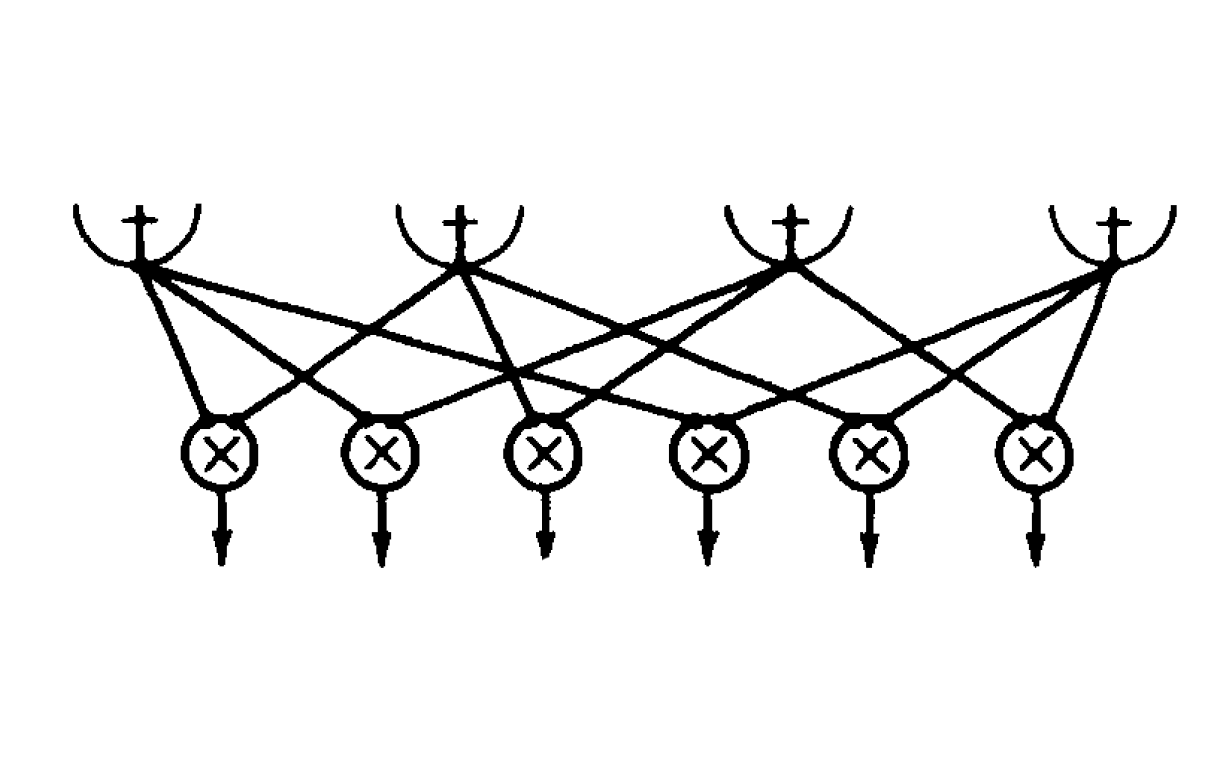
\includegraphics[scale= 0.2]{Figures/correlarray}
 	\caption[A correlator array   ]{A correlator array~\citep[Pg.~130,~Fig.~5.4(b)]{thompson2008interferometry}}
	\label{fig:correlArray}
\end{figure}
\subsubsection{Spatial Sensitivity and the Spatial Transfer function}
\label{sec:SsSt}
{\citep[From][Sec.~5.3]{thompson2008interferometry}}~We can now consider the sensitivity of an antenna array to the spatial frequencies on the sky. The angular response pattern see figure~\ref{fig:AntPat} of an antenna is the same in reception or transmission, so let's consider the antenna in transmission here, then the power applied to the terminals produces a field at the antenna aperture. A function $W(u,v)$ is equal to the autocorrelation function of $\pmb{\mathscr{E}}(x_\lambda{,y_\lambda})$, the distribution of the electric field across the aperture, where $x_\lambda$, and $y_\lambda$ are coordinates in the aperture plane of the antenna and are measured in wavelength, (this is similar to what we did for the Wiener-Khinchin relation in section~\ref{sec:about2} and if we apply the form of the cross-correlation eqs. in section~\ref{sec:crxcorrelabt} for an autocorrelation). Thus 
\begin{align}
W(u,v) &=&\pmb{\mathscr{E}}(x_\lambda{,y_\lambda})\star{\star}{\,}\pmb{\mathscr{E}}(x_\lambda{,y_\lambda})& \nonumber \\
W(u,v) &= \int^{\infty}_{-\infty}\int^{\infty}_{-\infty}&\pmb{\mathscr{E}}(x_\lambda{,y_\lambda})\pmb{\mathscr{E}}^{\ast}(x_\lambda - u {,y_\lambda} - v)dx_\lambda{dy_\lambda}&
\end{align}
$W(u,v)$ is a very useful or important function, it is proportional to the number of ways, suitably weighted by the field intensity, in which a specific spacing vector $(u,v)$ can be found within the antenna aperture. In reception it is a measure of the sensitivity of the antenna to different spatial frequencies, this is why $W(u,v)$ is also referred to as the transfer function. If we consider the response of the array to a \textbf{point source} as for a point source the visibility is constant over the whole $(u,v)$ plane, the measured spatial frequencies are proportional to $W(u,v)$. Thus the point source response ${\mathcal{A}}(l,m)$ is the Fourier transform of $W(u,v)$. Where ${\mathcal{A}}(l,m) = A(-l,-m)$ but as the function is usually symmetrical it is not of great practical importance here.\\
\begin{figure}[htbp]
\center
    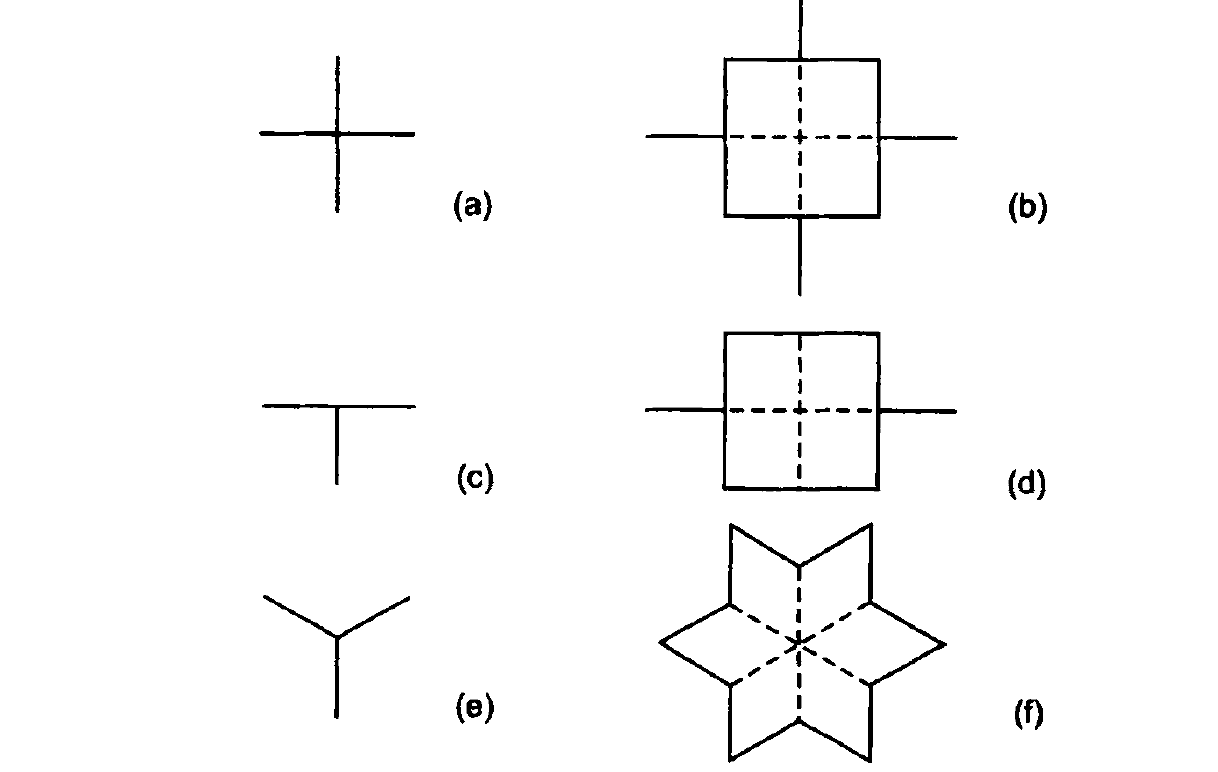
\includegraphics[scale= 0.2]{Figures/antconf}
 	\caption[Antenna aperture configurations and autocorrelation nonzero boundaries  ]{Antenna apertures configuration and autocorrelation nonzero boundaries~\citep[Pg.~136,~Fig.~5.7]{thompson2008interferometry}}
	\label{fig:antConf}
\end{figure}
Figure ~\ref{fig:antConf} shows some commonly used configurations of antenna arrays see fig.~\ref{fig:antConf} {\color{blue}(a),(c),(e)}, and the boundaries {\color{blue}(b),(d),(f)} of their autocorrelation functions. The autocorrelation function indicate the instantaneous spatial sensitivity for a continuous aperture in the form of the corresponding figure. Ridges of high autocorrelation are emphasised by the broken lines. These occur for displacements at which the arms of figures such
as those in Figure~\ref{fig:antConf} are aligned. 

A cross and its autocorrelation function are shown in Fig.~\ref{fig:antConf}{\color{blue}(a)} and {\color{blue}(b)}. It is assumed that the width of the arms is finite but small compared with the length of the arms. The spatial sensitivity is represented by the square in~\ref{fig:antConf}{\color{blue}(b)}. Notice the narrow extensions on the centres of the sides of the square represent parts of the autocorrelation functions of the individual arms, which are not formed in the cross-correlation of the arms. However, they are formed if the arms consist of lines of individual antennas for which the cross-correlation is formed for pairs on the \textbf{same arm} as well as those on crossed arms. The case for a T-shaped array is similar and is shown in Fig.~\ref{fig:antConf}{\color{blue}(c)} and {\color{blue}(d)}. Again, if only the cross-correlation between the east-west arm and the half-length, north-south arm is formed, then the spatial frequency coverage is represented by the square component of the autocorrelation. The equivalence between
the spatial transfer function of such a cross and a T can be understood by noting that for any pair of points in the aperture of a cross, for example, one on the east arm and one on the north arm, there is a corresponding pair on the west and south arms for which the spacing vector is identical. Thus any one of the four half-length arms can be removed without reducing the $(u,v)$ coverage of the spatial transfer function.

An alike example of a non-tracking T configuration is, the Mauritius Radio Telescope, near Bras d’eau, Mauritius, which was a T-shaped array of helix antennas operating at 150 MHz. The east-west arm is 2 km long. The south arm is 880 m long and was synthesised by moving a group of antennas on trolleys in steps, with continuous coverage, to simulate a larger aperture. The spatial frequency coverage is the same as would be obtained in a single observation with an antenna of aperture equal to that simulated by the movement of the antennas, although the magnitude of the spatial sensitivity is not exactly the same~{\citep[Sec.~5.6~Pg.~155,~Sec.~5.3~Pg.~137]{thompson2008interferometry}}.

Now consider the case of a tracking array, as the source moves in hour angle, the changing $(u,v )$ coverage is represented by a band centred on the spacing locus of the two antennas. Since $V(-u,-v) = V^{*}(u,v)$, any pair of antennas measures visibility along two arcs symmetric about the $(u,v)$ origin, both of which are included in the spatial transfer function. Because the antennas track the source, the antenna beams remain centred on the same point in the source under investigation, and the array measures the product of the source intensity distribution and the antenna pattern. 

To accommodate the effects that result when the antennas track the source position, the normalised antenna pattern is treated as a modification to the intensity distribution, the intensity distribution then becomes $A_N(l,m)I(l,m)$. The spatial transfer function $W(u,v)$ for a pair of tracking antennas is represented at any instant by a pair of two-dimensional delta functions
$\delta(u, v )$ and $\delta^{\ast}(-u,-v)$. For an array of antennas the resulting spatial transfer function is represented by a series of delta functions weighted in proportion to the magnitude of the instrumental response. As the earth rotates, these delta functions generate the ensemble of elliptical spacing loci. The loci represent the spatial transfer function of a tracking array.

Consider observation of a source $I(l,m)$, for which the visibility function is $V(u ,v)$, with normalised antenna patterns $A_N(l,m)$. Then if $W(u ,v)$ is the spatial transfer function, the measured visibility is 
\begin{equation}
\label{eq:measVis}
[V(u,v)\ast{\ast}{\,}\overline{A_N}(u,v)]W(u,v)
\end{equation}
where the double asterisk indicates two-dimensional convolution and the bar denotes the Fourier transform. The Fourier transform of~\ref{eq:measVis} gives the measured intensity:
\begin{equation}
\label{eq:measInt}
[I(l,m){A}_N(l,m)]\ast{\ast}{\,}\overline{W}(l,m)
\end{equation}
If we observe a \textbf{point source} at the $(l,m)$ origin, where ${A}_N = 1$, expression~\ref{eq:measInt} becomes the point-source response $b_0(l,m)$ . We then obtain

\begin{equation}
\label{eq:mBeam}
b_0(l,m)=[\delta(l,m){A}_N(l,m)]\ast{\ast}{\,}\overline{W}(l,m) = \overline{W}(l,m)
\end{equation}

where $\delta(l,m)$ represents the point source. Here again, the point-source response is the Fourier transform of the spatial transfer function. In the tracking case the spatial frequencies that contribute to the measurement are represented by ${W}(u,v)\ast{\ast}{\,}\overline{A_N}(u,v) $. We also note that $\overline{A_N}(u,v)$ is twice as wide as the corresponding antenna aperture in the $(x,y)$ domain.

As a first step in considering the layout of the antennas it is useful to consider
the desired spatial $(u,v)$ coverage. For any specific observation,
the optimum $(u,v)$ coverage clearly depends on the expected intensity distribution of the source under study, since one would prefer to concentrate
the capacity of the instrument in $(u,v)$ regions where the visibility is nonzero. However, most large arrays are used for a wide range of astronomical objects, so some compromise approach is required. Since, in general, astronomical objects are aligned at random in the sky, there is no preferred direction for the highest resolution. Thus it is logical to aim for visibility measurements that extend over a circular area centred on the $(u,v)$ origin. As described in Section 5.2, the visibility data are usually interpolated onto a rectangular grid for convenience in Fourier transformation, and if approximately equal numbers of measurements are used for each grid point, they can be given equal weights in the transformation. Uneven weighting results in loss of sensitivity, since some values then contain a larger component of noise than others. From this viewpoint one would like the natural weighting (i.e., the weighting of the measurements that results from the array configuration without further adjustment) to be as uniform as possible within the circular area.

Consider a circular $(u,v)$ area of diameter $a_\lambda$ wavelengths in which there are no holes in the data; that is, the visibility data interpolated onto a rectangular grid for Fourier transformation has no missing values. Then for uniform weighting, the synthesised beam, which is obtained from the Fourier transform of the gridded transfer function has the form of the following bessel function, $J_1(\pi{a_\lambda{\theta}})/\pi{a_\lambda{\theta}}$. Let us refer to the $(u,v)$ area described above as the complete $(u,v)$ coverage and the resulting beam as the complete response. Now if some data are missing, the actual $(u,v)$ coverage is equal to the complete coverage minus the $(u,v)$ hole distribution. By the additive property of Fourier transforms, the corresponding synthesised beam is equal to the complete response minus the Fourier transform of the hole distribution. The holes add an unwanted component to the complete response, in effect adding sidelobes to the synthesized beam.\\


To wrap up this section, the following illustrations in Fig.~\ref{fig:weighting2} will help us appreciate how the $(u,v)$ map coverage results in more information about the Intensity distribution  
\begin{figure}
        \centering
        \begin{subfigure}[b]{0.5\textwidth}
                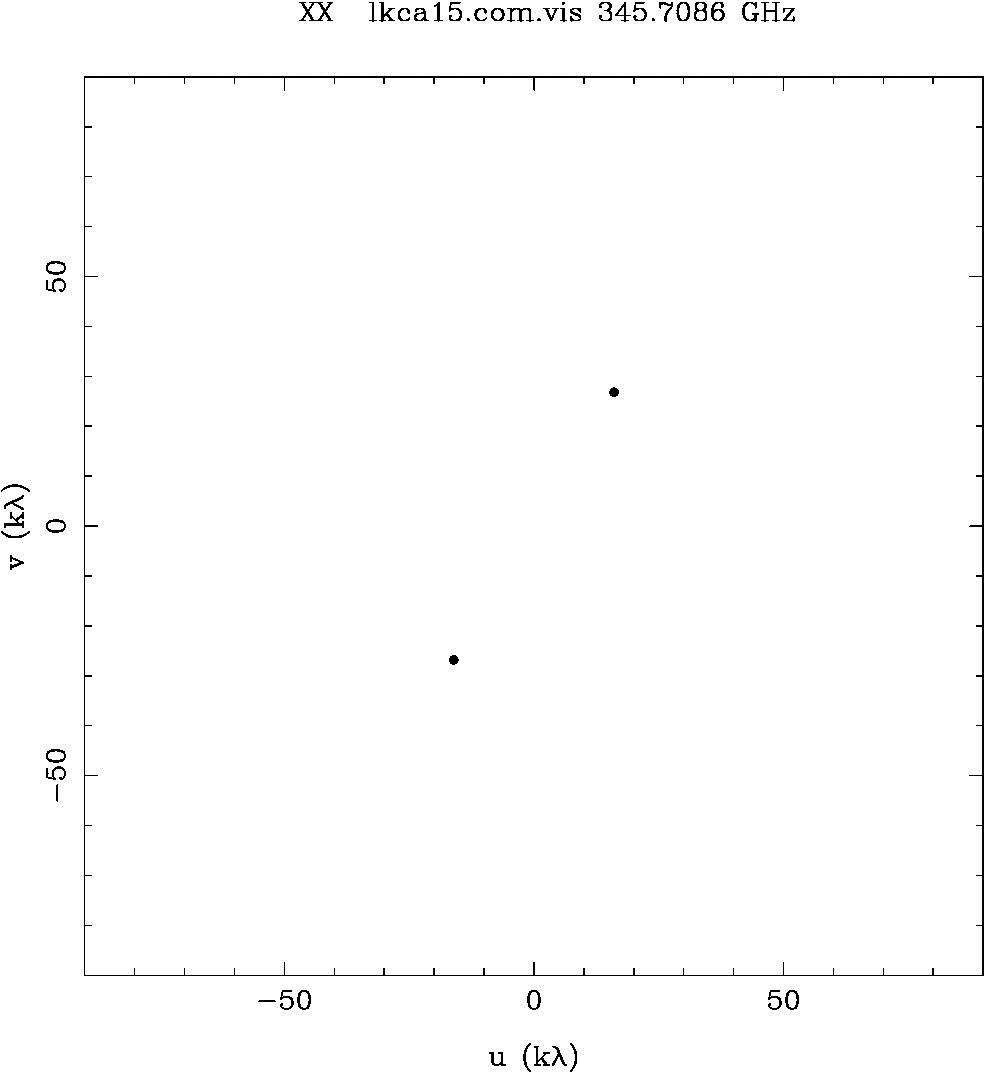
\includegraphics[scale=0.4]{Figures/uv-coverage/1antcov}
                \caption{$u-v$ coverage with 1 antenna - 2 samples}
                \label{fig:uv1ant}
        \end{subfigure}%
        ~ %add desired spacing between images, e. g. ~, \quad, \qquad, \hfill etc.
          %(or a blank line to force the subfigure onto a new line)
        \begin{subfigure}[b]{0.5\textwidth}
                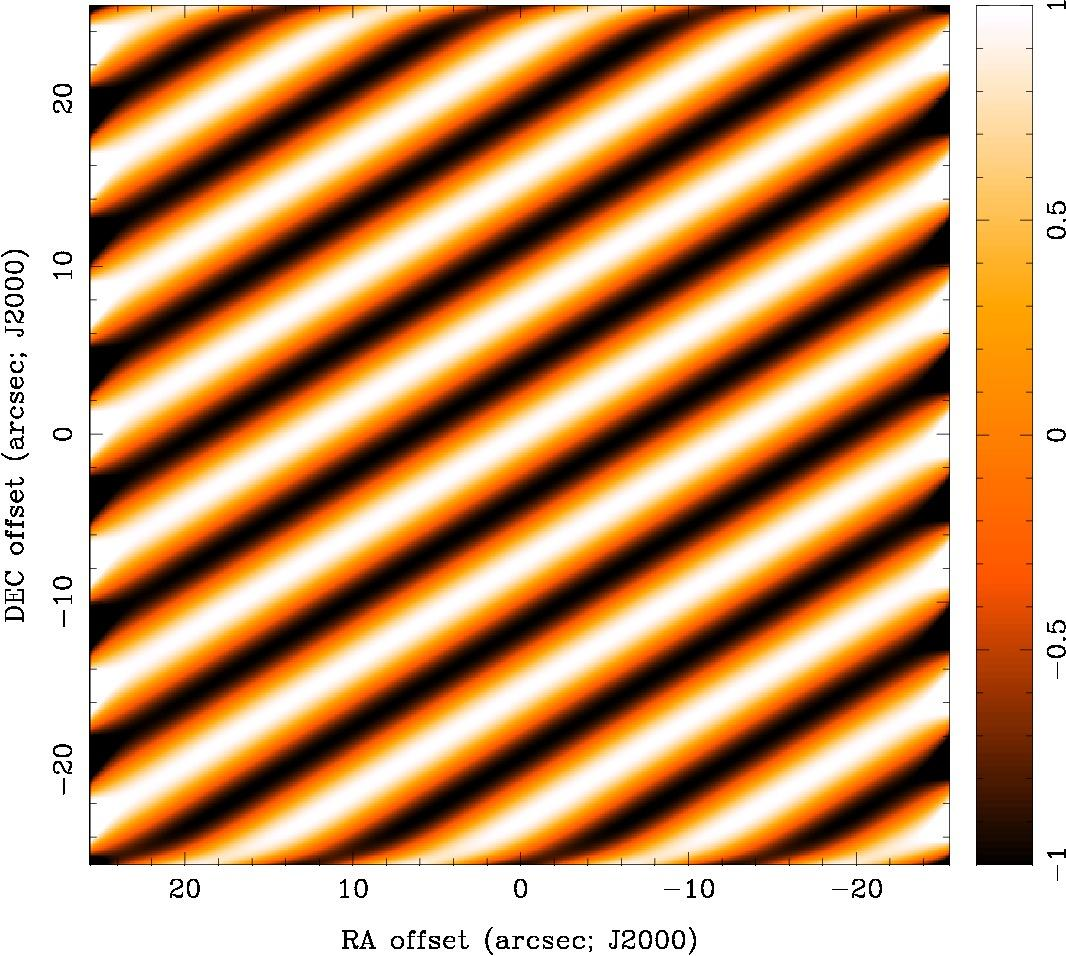
\includegraphics[scale=0.4]{Figures/uv-coverage/1antIma}
                \caption{Intensity map with 1 antenna - 2 samples}
                \label{fig:lm1ant}
        \end{subfigure} %
        %
        \begin{subfigure}[b]{0.5\textwidth}
                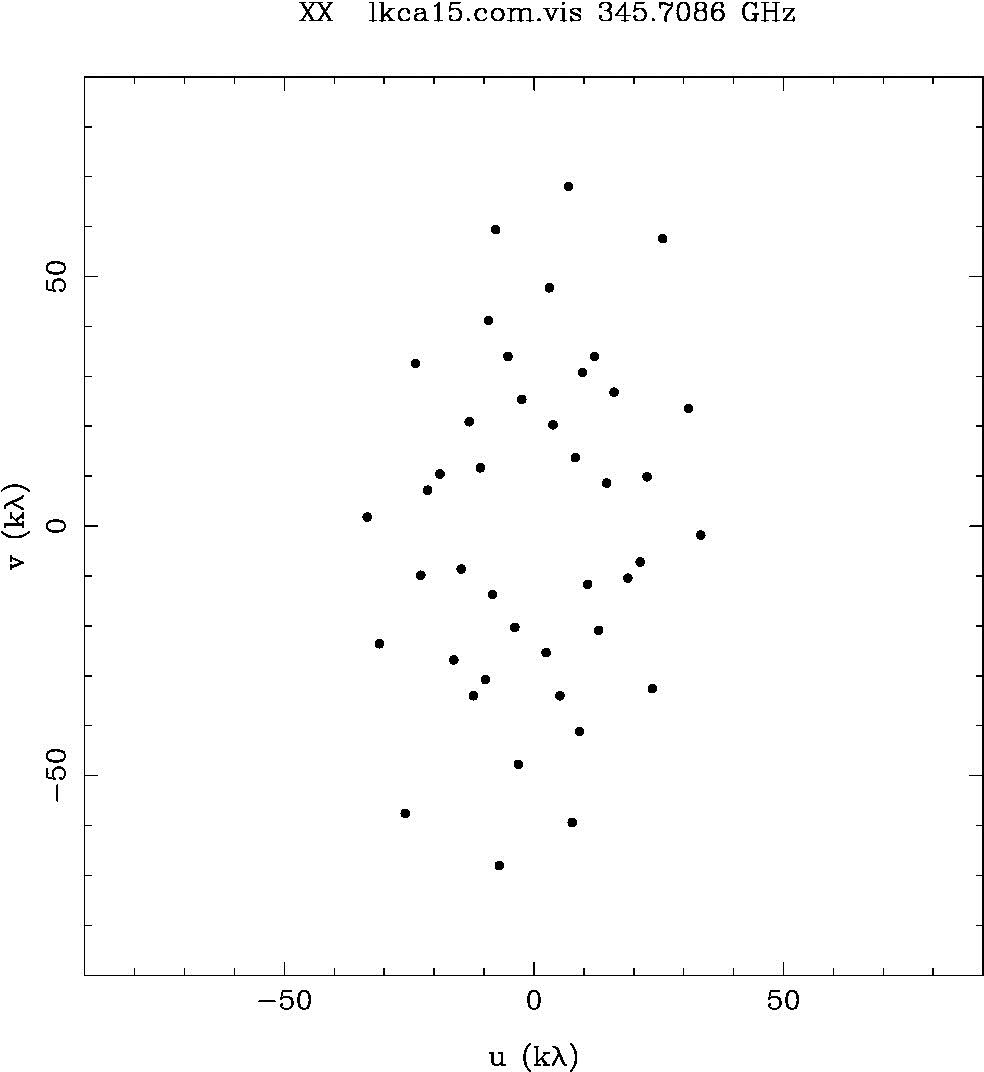
\includegraphics[scale=0.4]{Figures/uv-coverage/7antcov}
                \caption{$u-v$ coverage with 7 antennas\\ -- 7*6 = 42 samples}
                \label{fig:uv7ant}
        \end{subfigure}%
        ~ %add desired spacing between images, e. g. ~, \quad, \qquad, \hfill etc.
          %(or a blank line to force the subfigure onto a new line)
        \begin{subfigure}[b]{0.5\textwidth}
                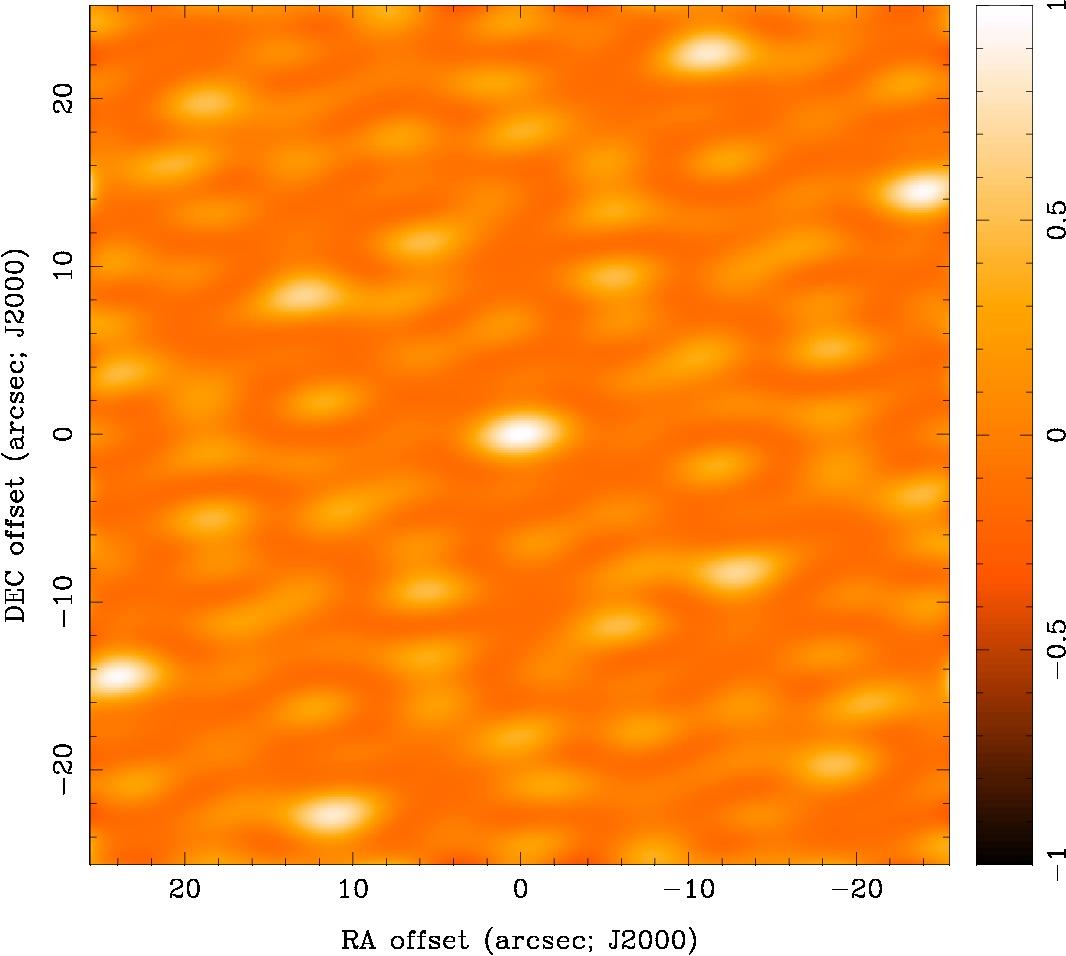
\includegraphics[scale=0.4]{Figures/uv-coverage/7antIma}
                \caption{Intensity map with 7 antennas\\ -- 42 samples}
                \label{fig:lm7ant}
        \end{subfigure} %
          \begin{subfigure}[b]{0.5\textwidth}
                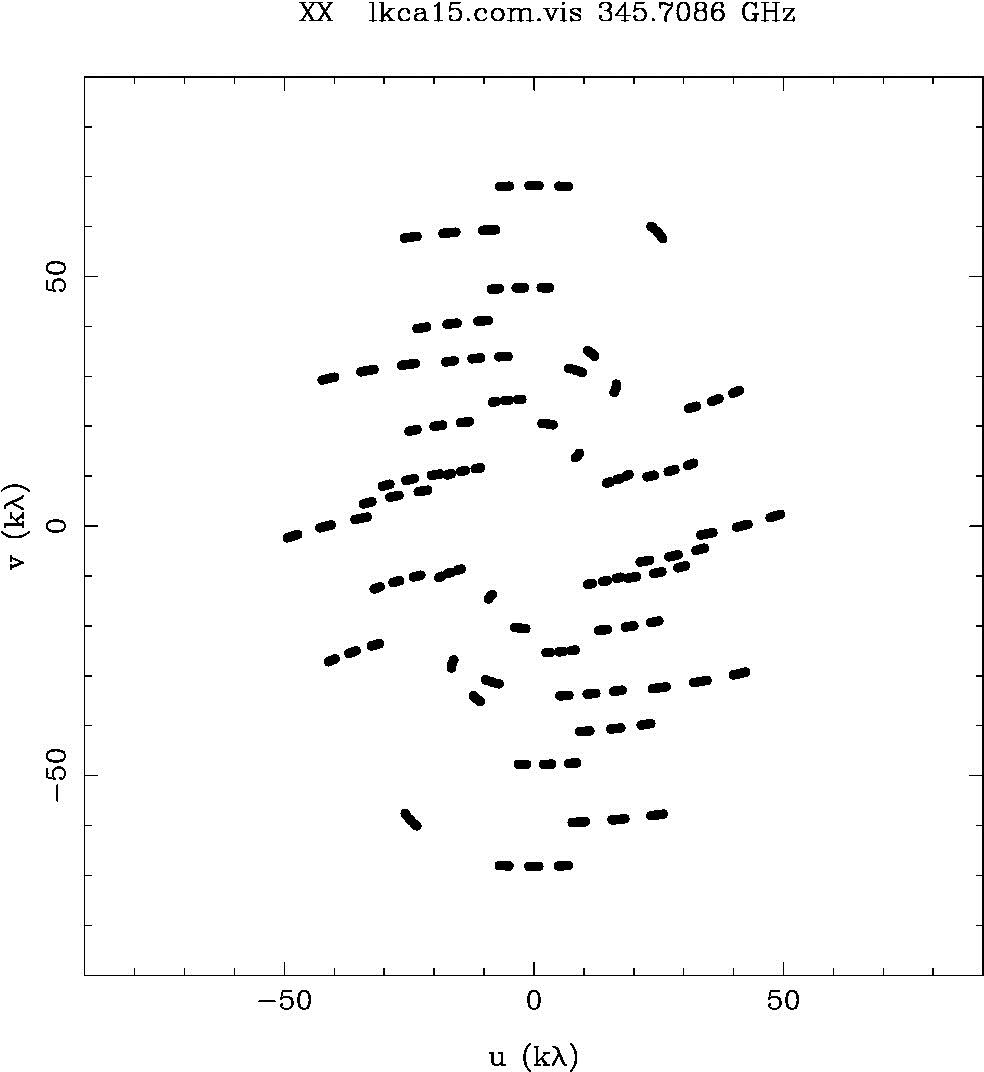
\includegraphics[scale=0.4]{Figures/uv-coverage/7antcov1h}
                \caption{$u-v$ coverage with 7 antennas - 1 hour}
                \label{fig:uv7ant1h}
        \end{subfigure}%
        ~ %add desired spacing between images, e. g. ~, \quad, \qquad, \hfill etc.
          %(or a blank line to force the subfigure onto a new line)
        \begin{subfigure}[b]{0.5\textwidth}
                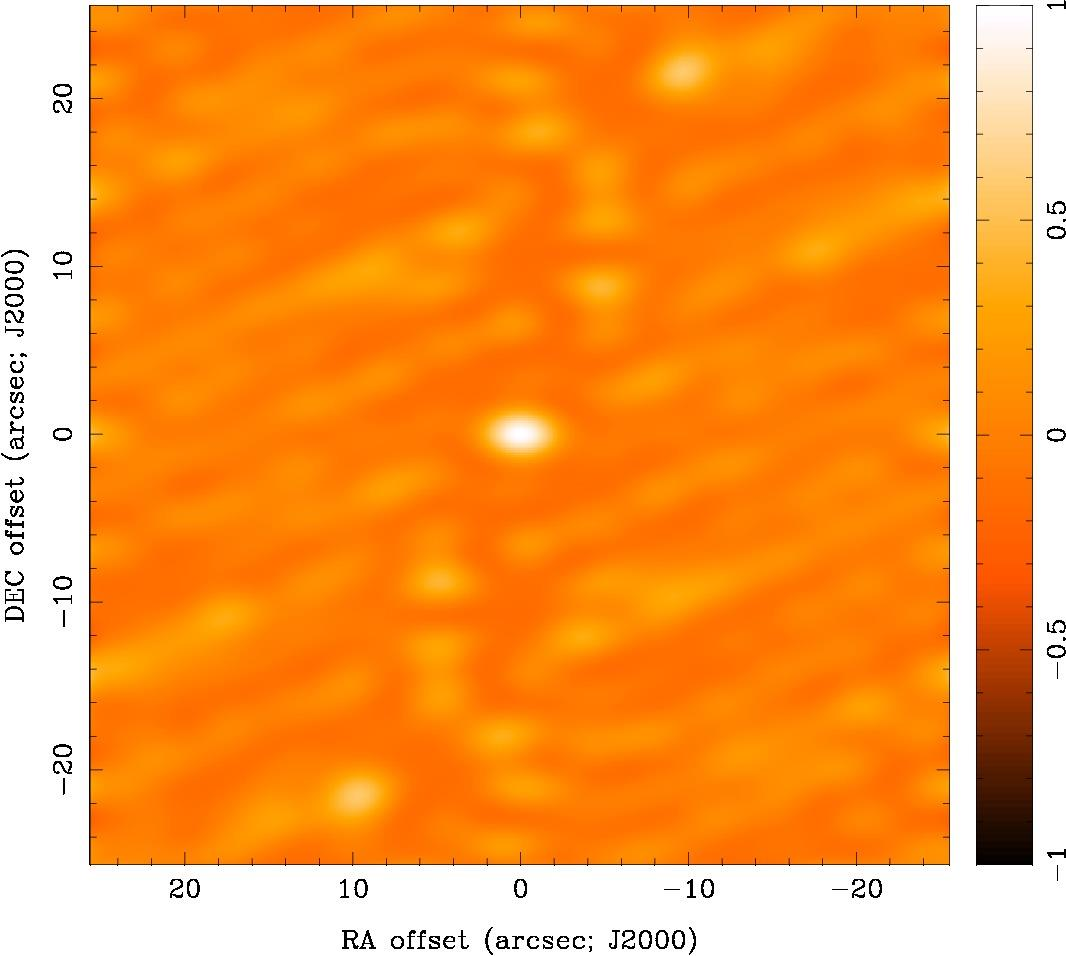
\includegraphics[scale=0.4]{Figures/uv-coverage/7antIma1h}
                \caption{Intensity map with 7 antennas - 1 hour }
                \label{fig:lm7ant1h}
        \end{subfigure}
        \begin{subfigure}[b]{0.5\textwidth}
                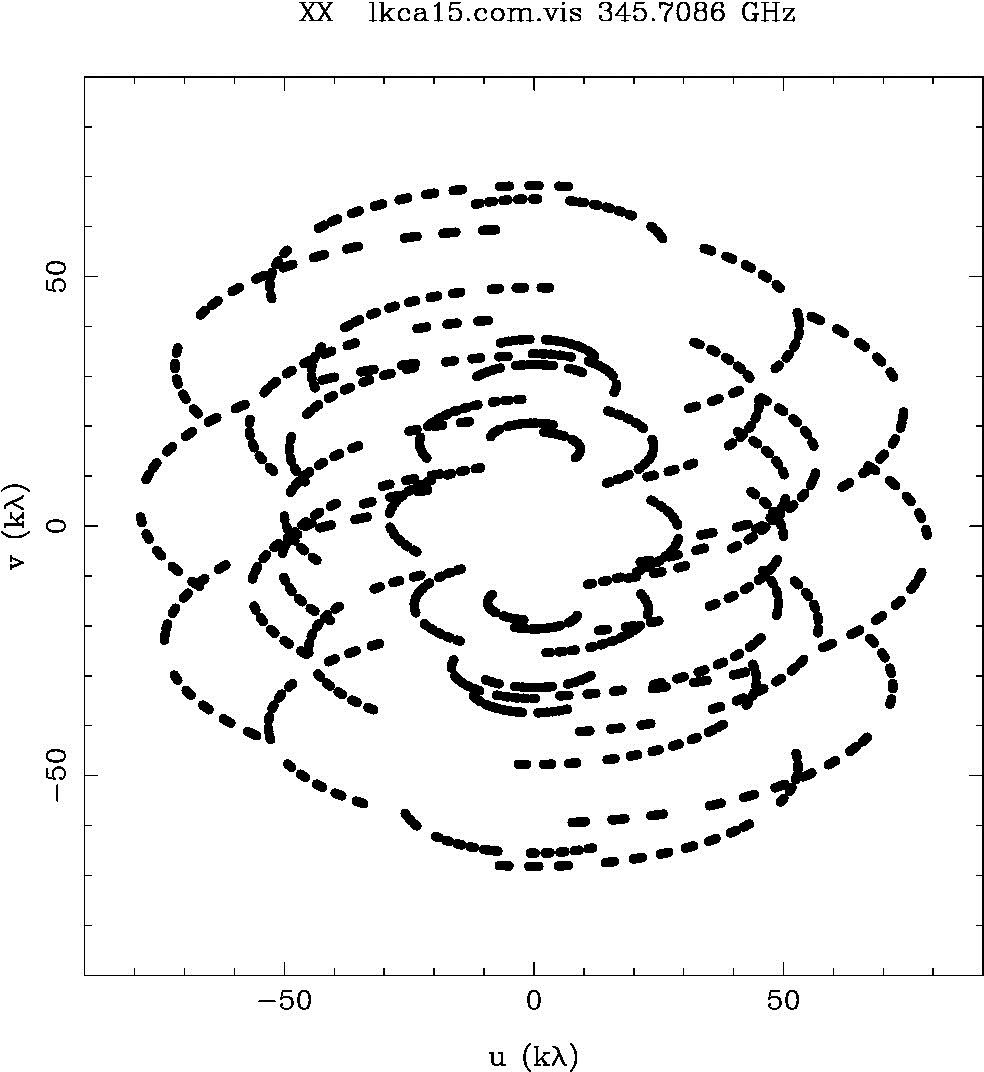
\includegraphics[scale=0.35]{Figures/uv-coverage/7antcov8h}
                \caption{$u-v$ coverage with 7 antennas - 8 hours }
                \label{fig:uv7ant8h}
        \end{subfigure}%%
        ~ %add desired spacing between images, e. g. ~, \quad, \qquad, \hfill etc.
          %(or a blank line to force the subfigure onto a new line)
        \begin{subfigure}[b]{0.5\textwidth}
                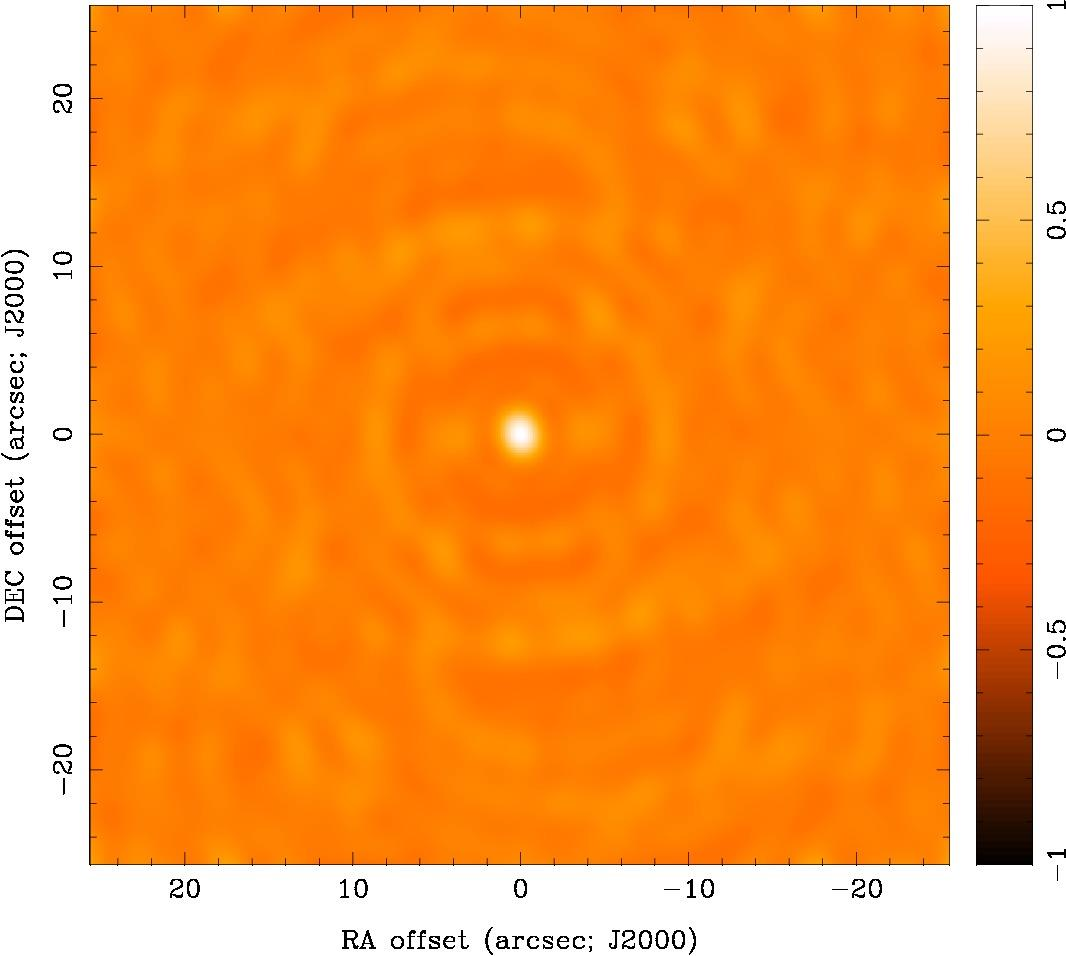
\includegraphics[scale=0.4]{Figures/uv-coverage/7antIma8h}
                \caption{Intensity map for 7 antennas - 8 hours}
                \label{fig:lm7ant8h}
        \end{subfigure}%%
        \caption[Visibility map coverage and derived Intensity map]{ Visibility map coverage and derived Intensity map~\citep[Slide 28,33,36,38]{wilner.siw2014}}\label{fig:weighting2}
\end{figure}
\newpage
\section{Data calibration}
{\citep[From][Sec.~10.1~Pgs.~383-385]{thompson2008interferometry}}~The aim of calibration is to remove, as much as possible, the effects of instruments and atmospheric factors in instruments. Such factors depend largely on the individual antennas or antenna pairs and their associated electronics, so a correction must be applied to the visibility data before they are combined into an image. Editing the visibility data to delete any that show evidence of radio interference or equipment malfunction is usually performed before the proper calibration. This mainly implies examining samples of data for unexpected levels or phase variations. Data taken on calibration sources are particularly useful here since the response to such a source is predictable and is expected to vary only slowly and smoothly with time.

First instrumental factors that are stable over periods of weeks or more are considered, there are also effects that vary during an observation and principally involves correction of the complex gain of the antenna pairs, these can be divided into two categories, the ones which can be predicted or measured and those which must be determined by observing a calibration source during the observation period.
\subsection{Calibration using calibration sources}
{~\citep[From][Sec.~10.1~Pgs.~385-387]{thompson2008interferometry}}~The steps in calibration involve parameters that may vary on timescales of minutes or hours and require the observation of one or more calibration sources. The source that is the subject of the astronomical investigation is referred as the target source to distinguish it from the calibration source, or calibrator. From Eq.~\ref{eq:visEq} we can write the expression for the interferometer response as follows:
\begin{equation}
\label{eq:vcal}
[V(u,v)]_{uncal} = G_{ik}(t) \int^{\infty}_{-\infty}\int^{\infty}_{-\infty}\frac{{A_N}(l,m)I(l,m)}{\sqrt{1 - l^2 - m^2}}e^{-j2\pi(ul + vm)}dldm
\end{equation}
Where, $[V(u,v)]_{uncal}$, is the uncalibrated visibility and, $I(l,m)$ is the source intensity. The complex gain factor $G_{ik}(t)$ is a function of the antenna pair $(i,k)$ and, as a result of unwanted effects, may vary over time. $A_N$ is the antenna aperture normalised to unity for the direction of the main beam. It can be removed from the source image as a final step in image processing and this is discussed in chapter~\ref{Chapter4}.  The factor ${A_N}(l,m)/{\sqrt{1 - l^2 - m^2}}$ in the intensity-{visibility} relationship is close to unity, and thus here on we shall omit it, except in the case of wide-field mapping that we won't cover in this report. To calibrate $G_{ik}(t)$, an unresolved calibrator can be observed for which the measured response is

\begin{equation}
\label{eq:calibVis}
V_c(u,v) = G_{ik}(t)S_c
\end{equation}

where the subscript, $c$, is to denote the calibrator and $S_c$ is the flux density of the calibrator. In calibrating it is best to consider the amplitude and phase separately, since the errors in these two quantities generally arise through different mechanisms. To calibrate the visibility of the target source we can thus write
\begin{equation}
\label{eq:Vcal}
V(u,v) = \frac{[V(u,v)]_{uncal}}{G_{ik}(t)} = [V(u,v)]_{uncal}\left[\frac{S_c}{V_c}\right]
\end{equation}

To observe the calibration source it is placed at the phase centre of its field. Then assuming that the calibrator is unresolved, the phase is a direct measure of the instrumental phase. Thus phase calibration for the target source simply requires subtracting the calibrator phase from the observed phase. The visibility amplitude can be calibrated using the moduli of the visibility terms in Eq.~\ref{eq:Vcal}. The response to the calibrator should be corrected for the calculable and/or directly monitored effects before the gain calibration is performed. Where there are separate receiving channels for two opposite polarizations at each antenna, the calibration must be performed separately for each one. For measurements of source polarization further calibration procedures are necessary which will not be discussed here.
The complex gain factor $G_{ik}(t)$ is of the antenna pair $(i,k)$ is indicated as follows,
\begin{equation}
\label{eq:Gain}
G_{ik}(t) = g_ig^{\ast}_k
\end{equation}

so the measured gains for antenna pairs can be used to determine gain factors for the individual antennas. Using the antenna gain factors rather than the baseline gain factors reduces the calibration data to be stored, and helps in monitoring the performance of individual antennas. Also, with this technique, some of the spacings can be omitted from the calibration observation so long as each of the antennas is included. In practice, gain tables including both amplitude and phase are generated for the antennas as a function of time, and the values are interpolated to the times at which data from the target source were taken. The interpolation should be done separately for the amplitude and phase, not for the real and imaginary parts of the gain, otherwise the phase errors can degrade the amplitude, and vice versa. The desirable characteristics of a calibration source are the following.
\begin{itemize}
\item Flux density -- The calibrator should be strong, so that a good signal-to-noise ratio is obtained in a short time, to reduce the $(u, v)$ coverage lost from the target source.
\item Angular width -- The calibrator should, if possible, be unresolved so that precise details of its visibility are not required.
\item Position -- The position of the calibrator should be close to that of the target source. Effects in the atmosphere or antennas that cause the gain to vary
with pointing angle are then more effectively removed, and time lost in
driving the antennas between the target source and calibrator positions is
kept small. 
\end{itemize}

It is not always possible to find a calibrator that satisfies all of the above requirements. In such cases it may be necessary to find a source that is largely unresolved and close to the target source, and then calibrate it against one of the more commonly used flux density references.

\section{Image Reconstruction}
{~\citep[From][Sec.~10.1~Pgs. 387-394]{thompson2008interferometry}}~The most straightforward method of obtaining an intensity distribution from measured visibility data is by direct Fourier transformation. The measured visibility $V_{meas}(u,v)$ can be written
\begin{equation}
\label{eq:measVisibi}
V_{meas}(u,v) = W(u,v)w(u,v)V(u,v),
\end{equation}
where $W(u,v)$ is the transfer function as introduced in the previous section~\ref{sec:SsSt}, and $w(u,v)$ represents any applied weighting. The Fourier transform of Eq.~\ref{eq:measVisibi} is the measured intensity distribution, which is 
\begin{equation}
\label{measIntensiti}
I_{meas}(l,m) = I(l,m)\ast{\ast}\,{b_0{(l,m)}},
\end{equation}
Where the double asterisk indicates convolution in 2-D and $b_0$ is the synthesised beam, which is the Fourier transform of the weighted transfer function:
\begin{equation}
b_0(l,m) \rightleftharpoons W(u,v)w(u,v)
\end{equation}

where, $\rightleftharpoons$, indicates the Fourier transform relationship. Effects such as non-coplanar baselines and others of minimal importance here and are not included. The visibility is measured at an ensemble of $n_d$ pairs of points symmetric about the $(u,v)$ origin, and the direct Fourier transform of these data is represented by
\begin{equation}
\sum^{n_d}_{i=1}w_i[ V_{meas}(u_i,v_i)e^{j2\pi(u_il+v_im)}V_{meas}(u_i,v_i)e^{-j2\pi(-u_il-v_im)}]
\end{equation}

 The weighting factor $w_i$ is introduced to control the form of the synthesized beam, $b_0(l,m)$. Since the visibility at $(-u_i,-v_i)$ is the complex conjugate of the visibility at $(u_i,v_i)$, the derived intensity is real (here we are considering the case where the antennas are identically polarized.)
 In the Fourier transformation of the visibility, the intensity is usually
computed at points in a rectangular grid with uniform increments in $l$ and $m$, since this is a very convenient form for subsequent processing.\\
\subsection{Weighting of the visibility}
To obtain the best signal-to-noise ratio in the summation of measurements that contain Gaussian noise, the individual data values should be weighted inversely as their variance, this is known as natural weighting, for most arrays though natural weighting results in poor beam shape because the shorter spacings are overemphasised. Thus the usual approach is to include in the weighting a factor that is inversely related to the area density of the data in the $(u,v)$ plane. By this mean we obtain data that has a uniform density. However with uniform weighting the strong, near-in sidelobes (close to the main beam) obscure low-level detail and thereby reduce the range of intensity levels that can be reliably measured. The near-in sidelobes of the functions can be reduced at the expense of some increase in the width of the synthesised beam by introducing a Gaussian or similar taper into the weighting function, and thus our resulting weighting function consists of the following
\begin{equation}
w(u,v) = w_u(u,v)\cdot{w_t(u,v)}
\end{equation}
$w_u(u,v)$ denotes weighting required to obtain uniform effective density, and ${w_t(u,v)}$ denotes the tapering function.
Thus the synthesised beam is the Fourier transform of $W(u,v)w_u(u,v){w_t(u,v)}$:
\begin{equation}
\label{eq:synthBeam}
b_0(l,m) = \overline{W}(l,m)\ast\ast{\,}\overline{w}_u(l,m)\ast\ast{\,}\overline{w}_t(l,m)
\end{equation}

\begin{figure}[h]
        \centering
        \begin{subfigure}[b]{0.3\textwidth}
                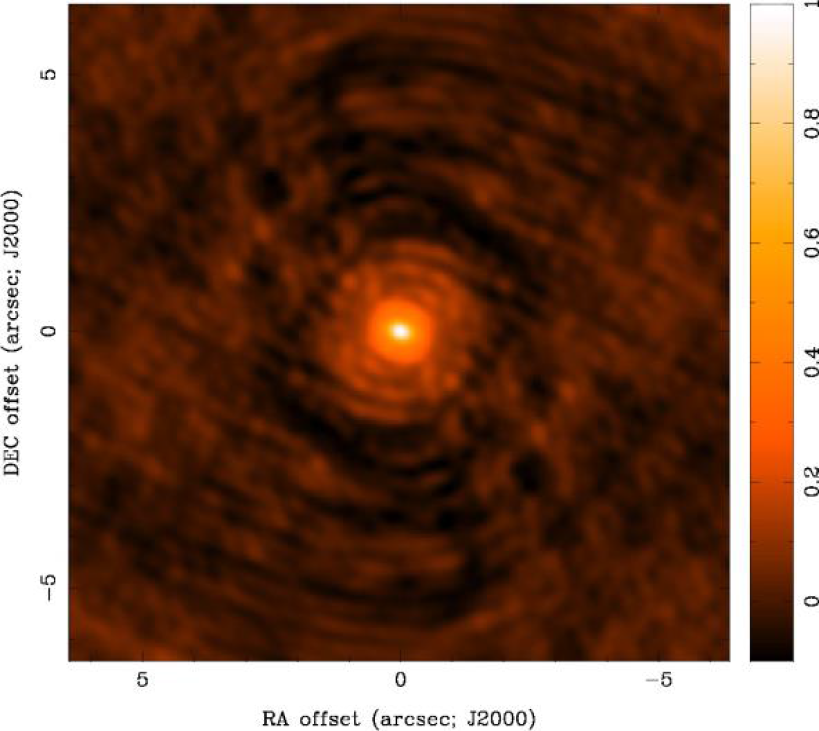
\includegraphics[width=\textwidth]{Figures/naturalWeight}
                \caption{The effect of natural weighting on the derived image}
                \label{fig:naturalWeight}
        \end{subfigure}%
        ~ %add desired spacing between images, e. g. ~, \quad, \qquad, \hfill etc.
          %(or a blank line to force the subfigure onto a new line)
        \begin{subfigure}[b]{0.3\textwidth}
                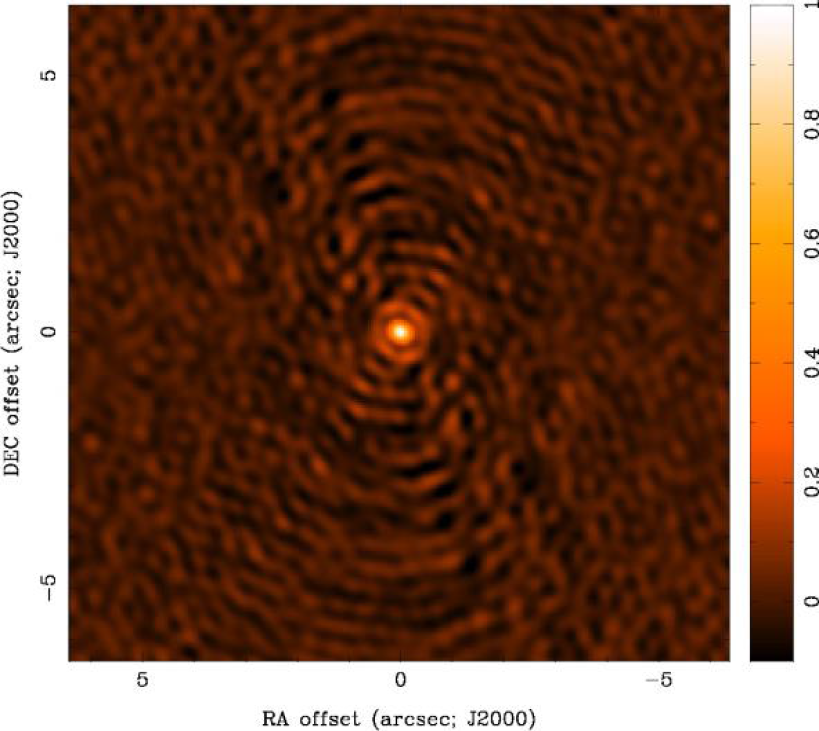
\includegraphics[width=\textwidth]{Figures/UniformWeight}
                \caption{The effect of uniform weighting on the derived image}
                \label{fig:UniformWeight}
        \end{subfigure}
        ~ %add desired spacing between images, e. g. ~, \quad, \qquad, \hfill etc.
          %(or a blank line to force the subfigure onto a new line)
           \begin{subfigure}[b]{0.3\textwidth}
                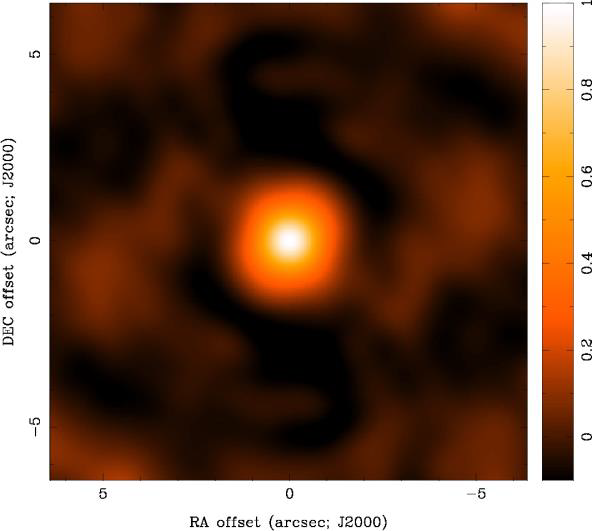
\includegraphics[width=\textwidth]{Figures/taper}
                \caption{The effect of the taper on the derived image\\ \hspace{10pt}}
                \label{fig:taper}
        \end{subfigure}
     
        \caption[The effect of weighting visibilities]{The effect of weighting visibilities~\citep[Slide 43,44,46]{wilner.siw2014}}\label{fig:weighting}
\end{figure}

where the bar denotes Fourier transform. One thing to note is that the Gaussian taper, $w_t(u,v)$ reduces the sidelobes outside of the main beam at the expense of widening the beam. 
\subsection{Mapping by Discrete Fourier transform}
As introduced in the section on sampling, section~\ref{sec:sampTheo}, the speed of the fast algorithm for the discrete Fourier transform (FFT) is a major advantage in computing large maps. However, the use of the FFT introduces two complications in addition to those discussed for the direct transform: (1) the necessity to evaluate the visibility at points on a rectangular grid and (2) the resulting possibility of aliasing of parts of the image from outside the synthesised field.
So again similarly one has to evaluate the visibility at the grid points, (to denote gridded maps we will use the supperscript,$^G$, hereafter,) the output of such a process can be expressed as follows: 
\begin{equation}
\label{eq:gridVis}
V^G(u,v) = w(u,v)\Sha_{(\Delta{u},\Delta{v})}(u,v)\left\lbrace{C(u,v)\ast{\ast}{\,}[W(u,v)\cdot{V(u,v)]}}\right\rbrace 
\end{equation}

Here the visibility $V(u,v)$, measured at the points denoted by the transfer function, $W(u ,v )$, is convolved with a function $C(u,v)$, to produce a continuous visibility distribution. This is then resampled at points in a rectangular grid with incremental spacings $\Delta{u}$ and $\Delta{v}$. This process is often referred to as \textbf{convolutional gridding}. The resampling is here represented by the two-dimensional impulse train function defined by,
\begin{equation}
\Sha_{(\Delta{u},\Delta{v})}(u,v) = \sum^{\infty}_{-\infty}\sum^{\infty}_{-\infty}\delta(u - i\Delta{u}, v - k\Delta{v}),
\end{equation}
where $\delta$ is the two-dimensional delta function. The weighting, $w(u,v)$ to optimize the beam is applied to the resampled data. In practice though, the convolution is evaluated only at the grid points. The Fourier transform of Eq.~\ref{eq:gridVis} represents the measured intensity:
\begin{equation}
\label{eq:gridInti}
I^{G}_{meas}(l,m) = \Sha_{(\Delta{u}^{-1},\Delta{v}^{-1})}(l,m)\ast{\ast}\,{\overline{w}(l,m)}\ast{\ast}\,{\left\lbrace{\overline{C}(l,m)[\overline{W}(l,m)\ast{\ast}{\,}{I(l,m)]}}\right\rbrace }
\end{equation}

As a result of the Fourier transformation, the intensity function $I(l,m)$ is convolved with the Fourier transform of the transfer function, multiplied by $\overline{C}(l,m)$ which is the Fourier transform of the convolving function, and then convolved with the Fourier transforms of the weighting and resampling functions. This last convolution, i.e. with $\Sha_{(\Delta{u}^{-1},\Delta{v}^{-1})}(l,m)$, causes the whole map to be replicated at intervals, $\Delta{u}^{-1}$ in $l$ and $\Delta{v}^{-1}$ in $m$. These intervals are equal to the dimensions of the map in the $(l, m )$ plane; that is, $\Delta{u}^{-1} = M\Delta{l}$ and $\Delta{v}^{-1} = N\Delta{m}$, for an $M \times N$ point array. The function $\overline{C}(l,m)$ takes the form of a taper applied to the map, and if this function does not vary greatly on the scale of the width of ${\overline{w}(l,m)}$ , which is usually the case for large maps, then ${\overline{w}(l,m)}$ in Eq.~\ref{eq:gridInti} can be convolved directly with
$\overline{W}(l,m)\ast{\ast}{\,}{I(l,m)}$, and Eq.~\ref{eq:gridInti} becomes
\begin{equation}
\label{eq:gridIntiApprox}
I^{G}_{meas}(l,m) \simeq \Sha_{(\Delta{u}^{-1},\Delta{v}^{-1})}(l,m)\ast{\ast}\,{\left\lbrace{\overline{C}(l,m)[{I(l,m)}\ast{\ast}{\,}b_0(l,m)]}\right\rbrace }
\end{equation}
where the synthesised beam $b_0(l,m )$ comes froms Eq.~\ref{eq:synthBeam},
However, the problem of aliasing remains, and the most effective way to deal with this is to convolve the data in the $(u ,v)$ plane with the Fourier transform of a function that, in the $(l,m)$ plane, varies very little over the map and then falls off rapidly at the map edges. We therefore look for a convolving function $C(u,v)$ for which the Fourier transform $I(l, m)$ has these properties, for example one could use of a Gaussian-Sinc function as the convolving function~({\citet[see][Sec.~10.2~Pgs. 394-399]{thompson2008interferometry}}).
